%%%%%%%%%%%%%%%%%%%%%%%%%%%%%% Preamble
\documentclass[11pt]{article}
\setlength{\parskip}{\baselineskip}%
\setlength{\parindent}{0pt}%
\usepackage{amsmath,amssymb,amsthm,physics,graphicx,titling,hyperref}
\usepackage[margin=0.5in]{geometry}
\newcommand{\subtitle}[1]{%
  \posttitle{%
    \par\end{center}
    \begin{center}\large#1\end{center}
    \vskip0.5em}%
}

\begin{document}

%%%%%%%%%%%%%%%%%%%%%%%%%%%%%% Heading
	\title{Ph 21.2 - Introduction to Fourier Transforms}
	\author{Yovan Badal}
	\date{04/14/2018}
	\maketitle
	
%%%%%%%%%%%%%%%%%%%%%%%%%%%%%% Body
\section{Properties and Consistency of the Fourier Series}
\begin{enumerate}
	\item We prove the consistency of eqns (2) and (3) as respective definitions of the inverse Fourier series and Fourier series.
	\begin{align}
		\sum_{k=-\infty}^{\infty} \tilde h_k e^{-2\pi i f_k x} =& \sum_{k=-\infty}^{\infty} e^{-2\pi i f_k x} \frac{1}{L} \int_0^L h(x')  e^{2\pi i f_k x'} \dd{x'} \\
		=& \int_0^L \sum_{k=-\infty}^{\infty} \frac{1}{L} h(x') e^{-2\pi i \frac{k}{L} (x'-x)} \dd{x'} \\
		=& \int_{-\infty}^{-\infty} \int_{-\infty}^{\infty} \frac{1}{L} h(x') e^{-2\pi i \frac{k}{L} (x'-x)} \dd{k} \dd{x'} \\
		=& \int_{-\infty}^{-\infty} h(x') \int_{-\infty}^{\infty} e^{-2\pi i k' (x'-x)} \dd{k'} \dd{x'} \\
		=& \int_{-\infty}^{-\infty} h(x') \delta(x'-x) \dd{x'} \\
		=& h(x)
	\end{align}
	where in line (3) we change the bounds of our $x$-integral by setting for convenience our function $h(x)$ to be $0$ outside of $x \in [0,L)$ and we use the fact that the signal we are concerned with is periodic to replace the infinite sum over $k$ with an indefinite k-integral. This is because the Fourier \textit{transform}, given by $H(k)=\int_{-\infty}^{\infty} h(x) e^{2 \pi i k x}\dd{x}$ (an extension of sorts of the Fourier series used to analyze aperiodic signals) of a periodic signal $h(x)$ consists of a sum of delta-distributions, which reduces the integral $H(k)$ to an infinte sum of complex exponetials over integer $k$. In line (4), we use a simple change of variables, in line (5) we use the Fourier transform of the dirac-delta distribution, and in line (6) we use the fundamental property of the dirac-delta distribution.
	
	\newpage
	\item We work out a special case of the completeness of complex exponentials.
	\begin{align}
		A\sin (2 \pi x/L + \varphi) &= \frac{i A}{2}(e^{-i(2 \pi x/L + \varphi)} - e^{i(2 \pi x/L + \varphi)}) \\
		&= \frac{i A}{2} \big(e^{-i \varphi} e^{-2 \pi i x/L} - e^{i \varphi} e^{2 \pi i x/L}\big) \\
		&= \bigg(\frac{i A}{2} e^{-i \varphi}\bigg) e^{-2 \pi i x/L} - \bigg(\frac{i A}{2} e^{i \varphi}\bigg) e^{2 \pi i x/L}
	\end{align}
	where in line (7) we have used DeMoivre's theorem. This proves the claim.
	
	\item We demonstrate a property of the Fourier coefficients for real $h(x)$.
	\begin{align}
		\tilde h_{-k} &= \frac{1}{L} \int_0^L h(x) e^{2 \pi i f_{-k} x} \dd{x} \\
		=& \frac{1}{L} \int_0^L h(x) e^{-2 \pi i f_{k} x} \dd{x} \\
		=& \frac{1}{L} \int_0^L h(x) \big[ e^{2 \pi i f_{k} x} \big]^{*} \dd{x} \\
		=& \bigg[ \frac{1}{L} \int_0^L h(x) e^{2 \pi i f_{k} x} \dd{x} \bigg]^{*} \\
		=& \tilde h_k^*
	\end{align}
	where in line (11) we have used the definition $f_k = \frac{k}{L}$, in line (12) we have used an obvious property of the complex exponential (which can easily be seen using DeMoivre's theorem) and in line (13) we have used the fact that $h(x)$ and our integration variable $x$ are real.
	
	\item We prove a version of the convolution theorem for Fourier series. Let $H(x) = h^{(1)}(x) h^{(2)}(x)$. Then we can write the Fourier series for $h^{(1)}(x)$ and $h^{(2)}(x)$:
	\begin{align}
	h^{(1)}(x) =& \sum_{k=-\infty}^{\infty} \tilde h_k^{(1)} e^{-2 \pi i f_k x} \\
	h^{(2)}(x) =& \sum_{k=-\infty}^{\infty} \tilde h_k^{(2)} e^{-2 \pi i f_k x}
	\end{align}
	such that we can write $H(x)$ as:
	\begin{align}
	H(x) =& h^{(1)}(x) h^{(2)}(x) \\
	=& \bigg( \sum_{k=-\infty}^{\infty} \tilde h_k^{(1)} e^{-2 \pi i f_k x} \bigg) \bigg( \sum_{k=-\infty}^{\infty} \tilde h_k^{(2)} e^{-2 \pi i f_k x} \bigg) \\
	=& \sum_{k=-\infty}^{-\infty} \bigg( \sum_{k'=-\infty}^{\infty} \tilde h_{k-k'}^{(1)} \tilde h_{k'}^{(2)} \bigg) e^{-2 \pi i f_k x}
	\end{align}
	and we can then find the Fourier coefficents $H_k$ of $H(x)$ as follows:
	\begin{align}
	H_k =& \frac{1}{L} \int_0^L H(x) e^{2 \pi i f_k x} \dd{x} \\
	=& \frac{1}{L} \int_0^L \sum_{l=-\infty}^{\infty} \bigg( \sum_{k'=-\infty}^{\infty} \tilde h_{l-k'}^{(1)} \tilde h_{k'}^{(2)} \bigg) e^{-2 \pi i f_l x} e^{2 \pi i f_k x} \dd{x} \\
	=& \frac{1}{L} \int_0^L \sum_{l=-\infty}^{\infty} \bigg( \sum_{k'=-\infty}^{\infty} \tilde h_{l-k'}^{(1)} \tilde h_{k'}^{(2)} \bigg) e^{2 \pi i (f_k - f_l) x} \dd{x} \\
	=& \frac{1}{L} \sum_{l=-\infty}^{\infty} \bigg( \sum_{k'=-\infty}^{\infty} \tilde h_{l-k'}^{(1)} \tilde h_{k'}^{(2)} \bigg) \int_0^L e^{2 \pi i (f_k - f_l) x} \dd{x} \\
	\end{align}
	Now, observe that $\int_0^L e^{2 \pi i (f_k - f_l) x} \dd{x} = \big\{_{0 \ \text{else}}^{L \ k=l}$ since we are integrating over an integer number of periods of the complex exponential. Therefore:
	\begin{align}
	H_k =& \sum_{k'=-\infty}^{\infty} \tilde h_{k-k'}^{(1)} \tilde h_{k'}^{(2)}
	\end{align}
	\textit{Graphical interpretation of the convolution product:} If we imagine a graphical interpretation of the \textit{spectrum} of a periodic function $h(x) = \sum_{k=-\infty}^{\infty} \tilde h_k e^{-2 \pi i f_k x}$ (the representation of the function $h(x)$ in $k$-space given by its Fourier series) as a graph of impulses ($\delta$-distributions) at $k$ scaled by $h_k$, we can represent the convolution product $H(x)$ as defined above as follows: we consider the spectrum of $h^{(1)}(x)$ (WLOG since convolution is clearly commutative by the above) as described above. We then consider the spectrum of $h^{(2)}(x)$, reflect it with respect to $k$ (i.e. $k \mapsto -k$) and offset it by $k'$ (i.e. $k \mapsto k + k'$). We then superpose the two spectra, multiply the scaling factors of the impulses superposed at every $k$, and sum the products over $k$ to obtain $H_{k'}$ (Note: in the limit of continuous spectra given by the Fourier transform, this sum becomes an integral represented in the above by the area under the product of the superposed spectra described above).
	
	\textit{Example (smooth $h_k^{(1)}$ centered at $k=0$, $h_k^{(2)} = \delta_{k, 50}$):}

\begin{figure}[!htbp]
  \begin{minipage}[b]{0.5\textwidth}
    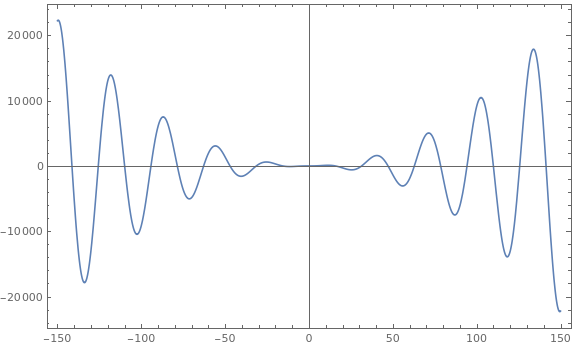
\includegraphics[width=\textwidth]{smooth_conv.png}
    \caption{$\tilde h_k^{(1)}$}
  \end{minipage}
  \hfill
  \begin{minipage}[b]{0.5\textwidth}
    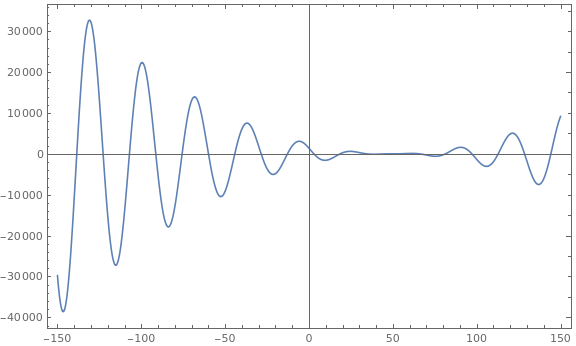
\includegraphics[width=\textwidth]{smooth_conv_shift.png}
    \caption{$\tilde H_k$}
  \end{minipage}
\end{figure}
	We observe that the convolution is simply the spectrum $h_k^{(1)}$ shifted forwards by 50 (i.e., $\tilde H_k$ = $h_{k-50}^{(1)}$).
\newpage

	\item 
\end{enumerate}
\end{document}